\chapter{Processi Markoviani}
\section{Processi stocastici}
Introdurremo dei modelli probabilistici che permettono di descrivere un mondo
che cambia nel corso del tempo. Per fare ciò, avremo bisogno di una serie di
variabili casuali descritte da uno stato che varia nel tempo. Le relazioni tra i
cambiamenti di stato nel tempo descrivono l'evoluzione della variabile.

Possiamo distinguere due tipologie di modelli:
\begin{itemize}
    \item \textbf{Statici}: il valore delle variabili non cambia nel tempo.
    \item \textbf{Dinamici}: il valore delle variabili cambia nel tempo. In questa
          tipologia, lo stato corrente dipende dalla storia e il processo di
          cambiamento è descritto da una serie di fotografie, o anche dette
          \textit{time slice}, ognuna delle quali contiene un insieme di variabili
          casuali.
\end{itemize}
\begin{definizione}[\textbf{Processo stocastico}]
    Un \textbf{processo stocastico} $\{X(t), t\in T\}$ è un insieme di variabili
    aleatorie che evolve nel tempo. Nello specifico, $X(t)$ rappresenta il valore
    della variabile aleatoria $X$ al tempo $t$.
\end{definizione}
Il tempo espresso dagli indici $t$ può essere continuo o discreto. Inoltre, tali
indici possono essere finiti o infiniti.

Avremo quindi diverse tipologie di processi stocastici:
\begin{itemize}
    \item Processi stocastici a tempo continuo:
          \begin{equation*}
              \{X(t), t>0\}
          \end{equation*}
    \item Processi stocastici a tempo discreto:
          \begin{equation*}
              \{X(t), t=0,1,\dots\}
          \end{equation*}
    \item Processi stocastici a stati continui:
          \begin{equation*}
              \{X(t), t=0,1,\dots\}, X(t) \text{ distribuzione continua}
          \end{equation*}
    \item Processi stocastici a stati discreti:
          \begin{equation*}
              \{X(t), t=0,1,\dots\}, X(t) \text{ distribuzione discreta}
          \end{equation*}
\end{itemize}
La variabile $X(t)$ rappresenta il valore della variabile dato dal sistema al
tempo $t$, cioè un valore che descrive uno stato del sistema al tempo $t$. Questo
stato può essere puntuale o cumulativo.
\begin{esempio}
    $X(t)$ può rappresentare il numero di visitatori fino al tempo $t$ (cumulativo),
    oppure può rappresentare il numero di visitatori al tempo $t$ (puntuale).
\end{esempio}
Un esempio di processo stocastico naive è il \textbf{random Walk}. Questo processo
vuole formalizzare l'idea di effettuare una camminata in cui la scelta del prossimo
passo è casuale. Può essere descritto attraverso la seguente equazione:
\begin{equation*}
    X(t) = X(t-1) + \varepsilon_t
\end{equation*}
dove $\varepsilon_t \in \{-1, 1\}$,  $P(\varepsilon_t = -1) = p$ e $P(\varepsilon_t = 1) = 1- p$.
Se $p=\frac{1}{2}$ allora il processo è bilanciato, altrimenti il modello verrebbe
chiamato random walk con \textbf{drift}, in quanto il processo tende a spostarsi
nella direzione più probabile.

Un modo per generalizzare questo processo è quello di esprimere la distribuzione
$\varepsilon_t$ come continua, ad esempio $\varepsilon_t \approx N(0, 1)$. Questo
crea una casualità maggiore.

Un'altro esempio di processo stocastico è il \textbf{processo autoregressivo del
    primo ordine} (\textit{first order autoregressive process}), il quale è descritto
dalla seguente equazione:
\begin{equation*}
    X_t = \alpha X_{t-1} + b + \varepsilon_t
\end{equation*}
con $\alpha,b$ constanti, con $-1<\alpha<1$ e $\varepsilon_t \approx N(0,1)$.

I processi stocastici sono importanti perché permettono di effettuare delle
predizioni, come ad esempio, il tracking degli oggetti in movimento nei video.
Oltre al tracking, possono essere utilizzati anche per generare dei processi come
la generazioni di comportamenti casuali per le simulazioni.
\section{Catene di Markov}
I processi stocastici possono rispettare una proprietà chiamata \textbf{proprietà
    Markoviana del primo ordine}, la proprietà assicura che la distribuzione di
probabilità per tutti i possibili valori futuri del processo dipende solo dal
valore corrente e non dai valori passati o da altre informazioni.

La generalizzazione di questa proprietà specifica il fatto che la distribuzione
di probabilità per tutti i possibili valori futuri del processo dipende da una
storia finita.

Tale proprietà può essere espressa in formule come:
\begin{equation}
    P(X_{t+1} = i_{t+1 } | X_t =i_t, \dots, X_{0} = i_{0})=P(X_{t+1} = i_{t+1 } | X_t =i_t)
\end{equation}
I processi stocastici che rispettano la \textbf{proprietà Markoviana} sono detti
\textbf{processi Markoviani} e verranno rappresentati attraverso una \textbf{catena di Markov}.

Quindi un processo stocastico a tempi discreti che rispetta la proprietà Markoviana
del primo ordine è una \textbf{catena di Markov del primo ordine} se per tutti
gli stati vale:
\begin{equation*}
    P(X_{t+1} = i_{t+1 } | X_t =i_t, \dots, X_{0} = i_{0}) = P(X_{t+1} = i_{t+1 } | X_t =i_t)
\end{equation*}
dove $P(X_0 = i_0) = q_i$, mentre $q = [q_1, \dots, q_i \dots q_n]$ rappresenta la
distribuzione di probabilità iniziale degli stati. Se non si conosce tale
distribuzione, si può assumere che sia uniforme.
\begin{nota}
    Quanto descritto fino a questo momento, può essere generalizzato a più ordini.
    Per fare ciò, si considera una storia di lunghezza pari all'ordine del processo.

    Possiamo dire che si vuole rispettare la proprietà Markoviana a più ordini.
\end{nota}
Questi processi si riferiscono a stati direttamente osservabili. Esistono anche
le catene associate a stati non osservabili direttamente, in questo caso si
parlerà di \textbf{catena di Markov nascoste}.

Se la probabilità di un certo evento è indipendente dal tempo $t$ la catena di
Markov si definisce \textbf{stazionaria} e si ha che:
\begin{equation}
    P(X_{t+1} = i_{t+1 } | X_t =i_t) = p_{ij}
\end{equation}
dove $p_{ij}$ specifica la probabilità di passare dal valore $X_t = i$ a $X_{t + 1} = j$.
\begin{nota}
    Una catena stazionaria \textbf{non} vuol dire che lo stato della variabile 
    rimane lo stesso nel tempo, ma che la probabilità di passare da uno stato 
    all'altro rimane costante.
\end{nota}

Quindi le catene di Markov possono essere rappresentate da una \textbf{matrice di
    transizione} (ad un passo), ovvero matrici quadrate di dimensione $n \times n$
con $n$ che rappresenta il numero di stati possibili.

Ogni elemento della matrice rappresenta la probabilità di passare da uno stato
all'altro.
\begin{equation*}
    P = \begin{bmatrix}
        p_{11} & p_{12} & \dots  & p_{1n} \\
        p_{21} & p_{22} & \dots  & p_{2n} \\
        \vdots & \vdots & \ddots & \vdots \\
        p_{n1} & p_{n2} & \dots  & p_{nn} \\
    \end{bmatrix}
\end{equation*}
La matrice ha i seguenti vincoli $p_{ij} \geq 0$ e $\sum_{j=0}^{n}p_{ij}=1, \forall i$.
\begin{nota}
    Per i modelli stazionari la matrice di transizione rimane identica nel tempo.
\end{nota}

La rappresentazione grafica di una \textbf{catena di Markov} è un grafo in cui i
nodi rappresentano gli stati che la variabile può assumere ($i,j,\dots$), mentre
gli archi rappresentano la probabilità di passare da uno stato all'altro. Quindi
la matrice di transizione diventa la matrice di adiacenza del grafo.
\begin{figure}[!ht]
    \centering
    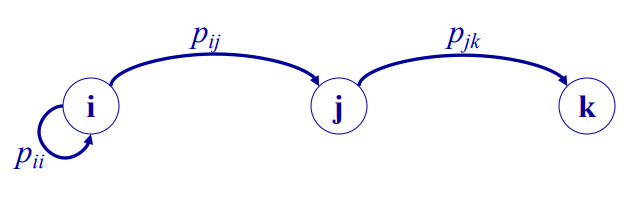
\includegraphics[width=0.5\textwidth]{img/catene/markovChain.png}
    \caption{Rappresentazione grafica di una catena di Markov}
    \label{fig:markovChain}
\end{figure}

A livello formale, per definire una \textbf{catena di Markov} devo avere:
\begin{itemize}
    \item Un insieme di stati $S = \{S_1, S_2, \dots, S_n\}$, ovvero i possibili
          valori che la variabile può assumere.
    \item La probabilità di transizione tra stati: $p_{ij} = P(X_{t+1} = S_i | X_t = S_j)$
    \item La distribuzione iniziale degli stati: $\pi_i = P[X_0 = S_i]$
\end{itemize}
Se non si conosce la distribuzione iniziale, allora si assume sia quella uniforme.
Mentre se si conosce con certezza il valore che assume la variabile all'inizio,
allora, considerando $i$ come il valore assunto da tale variabile, si avrà che:
\begin{equation*}
    \pi_i = 1, \forall j \neq i, \pi_j = 0
\end{equation*}
Per calcolare la \textbf{probabilità di una serie storica} mi basta effettuare
il prodotto della probabilità di ciascuno stato dato quello precedente, sfruttando
quindi la proprietà Markoviana.
\begin{esempio}
    Se vogliamo calcolare la probabilità della serie $Sn, R,R,R,Sw,Sw$, possiamo
    usare la seguente formula:
    \begin{equation*}
        P(\langle Sn, R,R,R,Sw,Sw \rangle) = P(Sn) \cdot P(R|Sn) \cdot P(R|R)
        \cdot P(R|R)\cdot P(Sw|R) \cdot P(Sw|Sw)
    \end{equation*}
    La probabilità iniziale $P(Sn) = \pi_{Sn}$, dove $\pi$ rappresenta la
    distribuzione iniziale della variabile aleatoria.
\end{esempio}
Quando la serie storica è molto lunga il prodotto tra probabilità tende a $0$,
quindi conviene passare al logaritmo.
\subsection{Inferenza}
Possiamo effettuare inferenza di valori per istanti di tempo più lontani.
Data la matrice di transizione, possiamo calcolare la probabilità che dopo $n$
passi si trovi in uno stato specifico $j$. Per fare ciò, dovremo calcolare:
\begin{equation}
    P(X_{m + n} = j | X_{m} = i) = P(X_n = j | X_0 = i)=p_{ij}(n)
\end{equation}
dove $p_{ij}(n)$ rappresenta la probabilità di passare dallo stato $i$ allo stato
$j$ in $n$ passi. Questa probabilità può essere calcolata attraverso la seguente
formula:
\begin{equation}
    p_{ij}(n) = \prod_{k = 1}^{n} p_{ij} \equiv p^n_{ij}
\end{equation}
ovvero, si calcola il prodotto riga per colonna della matrice di transizione
per $n$ volte. In questo modo, si considerano tutti i possibili percorsi che
portano dallo stato $i$ allo stato $j$ in $n$ passi.

La probabilità di transizione a $n$ passi
\begin{equation*}
    p_{ij}^n = P \left\{X_{n + k} = j | X_k = i\right\} \quad \text{con } n \geq 0
    , i, j \geq 0
\end{equation*}
può essere calcolata anche attraverso le equazioni di \textbf{Chapman-Kolmogorov}:
\begin{equation}
    p_{ij}^{n+m} = \sum_{k} p_{ik}^n \cdot p_{kj}^m \quad \text{con } n, m \geq 0, i, j \geq 0
\end{equation}
Questa formula permette di semplificare il calcolo della probabilità di transizione
a $n+m$ passi, affermando che essa è uguale alla somma delle probabilità di
transizione a $n$ passi moltiplicata per la probabilità di transizione a $m$ passi.
\begin{equation*}
    P^{n+m} = P^n \cdot P^m
\end{equation*}

La probabilità di essere in un certo stato $j$ al tempo $n$, non conoscendo lo
stato di una di una catena di Markov al tempo $0$, può essere calcolata attraverso
la seguente formula:
\begin{equation}
    \sum_{i} q_i \cdot p_{ij}^n = \vec{q} \cdot (\text{colonna j di } P^n)
\end{equation}
dove $q_i$ rappresenta la probabilità che la catena sia nello stato $i$ al tempo
$0$.

\begin{definizione}[\textbf{Raggiungibilità}]
    Uno stato $j$ è \textbf{raggiungibile} da uno stato $i$ se esiste un cammino
    che da $i$ arriva a $j$, in formule:
    \begin{equation*}
        P^n_{ij}>0
    \end{equation*}
    per qualche $n\geq 0$.
\end{definizione}
\begin{definizione}[\textbf{Comunicano}]
    Due stati $i$ e $j$ si dice che \textbf{comunicano} se $j$ è raggiungibile
    da $i$ e $i$ è raggiungibile da $j$. In formule:
    \begin{equation*}
        P^n_{ij}>0 \land P^n_{ji}>0
    \end{equation*}
    per qualche $n\geq 0$.
\end{definizione}
\begin{nota}
    Ogni stato comunica con se stesso per definizione e vale anche la proprietà
    transitiva.
\end{nota}
\begin{definizione}[\textbf{Irriducibilità}]
    Una catena di Markov è detta \textbf{irriducibile} se tutti i suoi stati sono
    comunicanti tra loro.
\end{definizione}
\begin{definizione}
    Un insieme di stati $S$ di una catena di Markov è un insieme \textbf{chiuso}
    se nessuno stato fuori $S$ è raggiungibile da stati in $S$.
\end{definizione}
\begin{definizione}[\textbf{Stato assorbente}]
    Uno stato $i$ si dice \textbf{assorbente} se $P_{ii} = 1$. Questo significa
    che una volta raggiunto lo stato $i$ non si può più uscire da esso.
\end{definizione}
\begin{definizione}[\textbf{Transiente}]
    Uno stato $i$ si dice \textbf{transiente} se esiste uno stato $j$ raggiungibile
    da $i$, ma $i$ non è raggiungibile da $j$. In formule:
    \begin{equation*}
        \sum_{n=1}^{\infty} P_{ii}^n < \infty
    \end{equation*}
\end{definizione}
\begin{definizione}[\textbf{Ricorrente}]
    Uno stato che non è transiente viene definito \textbf{ricorrente} se
    \begin{equation*}
        \sum_{n=1}^{\infty} P_{ii}^n = \infty
    \end{equation*}
\end{definizione}
\begin{nota}
    La ricorrenza è una proprietà di classe, se lo stato $i$ è ricorrente e
    lo stato $j$ comunica con $i$ allora $j$ è ricorrente.
\end{nota}
\begin{nota}
    Anche la transiente è una proprietà di classe.
\end{nota}
\begin{nota}
    Tutti gli stati di una catena di Markov \textbf{finita}, ovvero composta da
    un numero finito di stati, e \textbf{irriducibile} sono anche \textbf{ricorrenti}.
\end{nota}
\begin{definizione}[\textbf{Periodicità}]
    Uno stato $i$ è \textbf{periodico} di periodo $k > 1$ se $k$ è il più piccolo
    numero tale che tutti i cammini che dallo stato $i$ ritornano ad $i$ hanno una
    lunghezza che è multiplo di $k$.
\end{definizione}
\begin{definizione}[\textbf{Aperiodico}]
    Uno stato $i$ è \textbf{aperiodico} se non è \textit{periodico}.
\end{definizione}
\begin{definizione}[\textbf{Ergodicità}]
    Se tutti gli stati della catena di Markov sono \textbf{ricorrenti}, \textbf{aperiodici}
    e \textbf{comunicano} l'un con l'altro, la catena si definisce \textbf{ergodica}.
\end{definizione}
\begin{esempio}
    Un esempio di catena \textbf{ergodica} è quella riportata in figura \ref{fig:ergodic}.
    \begin{figure}[!ht]
        \centering
        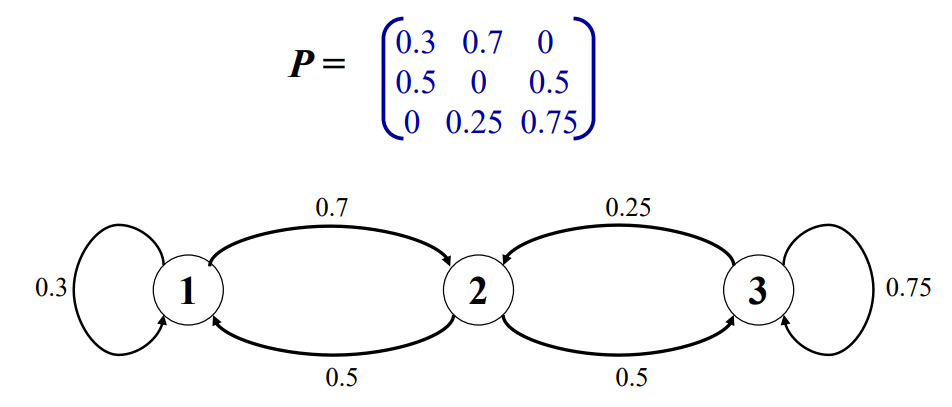
\includegraphics[width=0.5\textwidth]{img/catene/catena_ergodica.png}
        \caption{Esempio di catena ergodica}
        \label{fig:ergodic}
    \end{figure}
\end{esempio}

L'assunzione delle catene di Markov è che gli stati sono tutti direttamente osservabili,
il problema è che noi possiamo derivare la distribuzione delle variabili da delle
osservazioni su altre variabili del mondo. Significa che possiamo modificare la
distribuzione delle variabili non direttamente osservabili.
\section{Catene di Markov Nascoste}
L'evoluzione del mondo può essere modellata in modo più complesso, infatti possiamo
correggere le catene di Markov per rappresentare questa evoluzione:
\begin{itemize}
    \item $X_t$ insieme di variabili non osservabili al tempo $t$.
    \item $E_t$ insieme di variabili osservabili al tempo $t$.
    \item Dipendenze tra le variabili osservabili e non osservabili.
    \item Assunzione che i cambiamenti del mondo siano regolati da un processo
          stazionario.
    \item Assunzione di ipotesi di Markov (del primo ordine)
\end{itemize}
\begin{esempio}
    Il mio stato nascosto può essere pioggia o sole, ma non posso guardare fuori.
    Posso dedurre il tempo dalla presenza delle persone con l'ombrello bagnato o
    asciutto. Quindi osservare lo stato nascosto da altre variabili osservabili
    direttamente.
\end{esempio}
\begin{definizione}[\textbf{Catene di Markov a stati nascosti}]
    Le \textbf{catene di Markov a stati nascosti} sono un processo stocastico
    continuo/discreto caratterizzato da:
    \begin{itemize}
        \item $X_t$ insieme di stati nascosti al tempo $t$
        \item $E_t$ insieme di osservazioni al tempo $t$
        \item Matrice di probabilità di transizione
              \begin{equation*}
                  P(X_t | X_{0:t-1}) = P(X_t | X_{t-1})
              \end{equation*}
        \item Matrice di probabilità di emissione delle osservazioni (sono in uno
              stato allora qual è la probabilità di osservare qualcosa)
              \begin{equation*}
                  P(E_t | X_{0:t-1}, E_{0:t-1}) = P(E_t | X_{t})
              \end{equation*}
        \item Distribuzione delle probabilità a priori a $t=0$, $P(X_0)$.
    \end{itemize}
\end{definizione}
Il modello è caratterizzato da:
\begin{itemize}
    \item \textbf{Modello di transizione}: matrice di probabilità di transizione
          di dimensione $n\times n$ ($n$ numero di stati)
          \begin{equation*}
              P(X | X_{0:t-1}) = P(X | X_{t-1})
          \end{equation*}
    \item \textbf{Modello sensoriale}: matrice di probabilità di emissione delle
          osservazioni  $n\times m$ ($n$ numero di stati, $m$ numero di osservazioni)
          \begin{equation*}
              P(E | X_{0:t-1}, E_{0:t-1}) = P(E_{t} | X_{t})
          \end{equation*}
\end{itemize}
In generale, per ogni t finito, possiamo calcolare la distribuzione congiunta:
\begin{equation}
    P(X_0, x_1,\dots,X_t, E_1,\dots, E_t) = P(X_0) \prod_{i=1}^{t}P(X_i|X_{i-1}) \cdot P(E_i|X_i)
\end{equation}
\begin{nota}
    Pensare di utilizzare questo modello per effettuare il RL per il progetto di
    sistemi complessi.

    Utilizzare lo stesso metodo per predire gli attacchi.
\end{nota}
\begin{nota}
    Per calcolare le probabilità di entrambi i modelli si effettua un conto
    numerico dal dataset.
\end{nota}
Un esempio di grafico della catena nascosta \ref{fig:HMM}.
\begin{figure}[!ht]
    \centering
    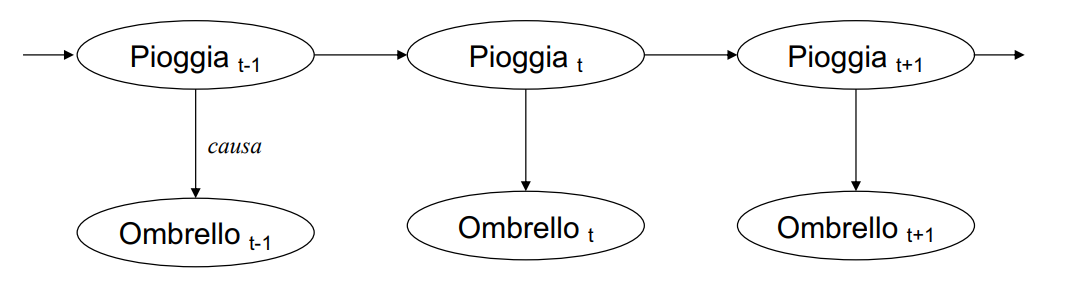
\includegraphics[width=.5\textwidth]{img/catene/hmm.png}
    \caption{Esempio di catena di Markov a stati nascosti}
    \label{fig:HMM}
\end{figure}

Secondo questo grafico potrebbero esserci problemi legati alla presenza di infinite
CPT, in realtà no perché si ha l'assunzione di \textbf{stazionarietà} (i cambiamenti
sono regolati da leggi immutabili nel tempo). In aggiunta si potrebbe pensare di
che ci siano infiniti genitori per ogni stato, in realtà no perché si ha l'assunzione
di \textbf{ipotesi di Markov} (lo stato corrente dipende solo da una storia finita
degli stati precedenti).

Si potrebbe pensare che l'\textbf{ipotesi di Markov} sia troppo stringente, per
rimediare possiamo aumentare l'ordine del modello di processo di Markov oppure di
aumentare l'insieme delle variabili di stato.
\subsection{Inferenza}
L'inferenza con questi modelli è di $4$ tipologie:
\begin{itemize}
    \item \textbf{Filtraggio}: calcolo $X_t$ dato tutte le osservazioni del
          passato $e_{1:t}$
          \begin{equation}
              P(X_t | e_{1:t})= f(e_t, P(X_{t-1}|e_{1:t-1}))
          \end{equation}
          In questo caso, le osservazioni partono da $1$, si può scegliere se
          raccoglierle da $1$ a $0$.

          Questa operazione è composta da due fasi:
          \begin{itemize}
              \item \textbf{Predizione}: calcolo della distribuzione dello stato
                    corrente al tempo $t$ dato l'osservazione fino al tempo $t-1$
                    \begin{equation}
                        P(X_t | e_{1:t-1})
                    \end{equation}
              \item \textbf{Aggiornamento}: calcolo della distribuzione dello stato
                    corrente al tempo $t$ data l'osservazione al tempo $t$:
                    \begin{equation}
                        P(e_t | X_{t})
                    \end{equation}
          \end{itemize}
          Queste due operazioni vengono unite in un unica formula:
          \begin{equation}
              P(X_{t} | e_{1:t}) = \alpha P(e_{t}|X_{t})\cdot P(X_{t}|e_{1:t-1})
          \end{equation}
          dove $\alpha$ è una costante di normalizzazione.

          La formula si ottiene prima separando l'evidenza al tempo $t$
          rispetto al tempo $t - 1$:
          \begin{equation*}
              P(X_{t} | e_{1:t}) = P(X_{t} | e_{1:t - 1}, e_{t})
          \end{equation*}
          Successivamente, utilizzando la regola di Bayes si riscrive la formula:
          \begin{equation*}
              P(X_{t} | e_{1:t - 1}, e_{t}) = \alpha P(e_{t}|X_{t}, e_{1:t-1})\cdot P(X_{t}|e_{1:t-1})
          \end{equation*}
          Infine, attraverso l'assunzione di indipendenza tra $e_{t - 1}$ e $e_{t}$
          otteniamo la formula finale.
    \item \textbf{Previsione}: coincide col filtraggio privo della fase di
          aggiornamento attraverso le osservazioni. Coincide col calcolare:
          \begin{equation}
              P(X_{t+k } | e_{1:t}) = \sum_{x_t} P(X_{t+k}|x_t) P(x_t)
          \end{equation}
          Più allunghiamo l'orizzonte di previsione, più l'incertezza aumenta,
          più breve sarà il tempo per raggiungere un punto fisso per una predizione
          (distribuzione stazionaria) e più ignoto sarà il futuro.

          Possiamo usare una ricorsione per il calcolo della verosimiglianza di
          una sequenza di osservazioni:
          \begin{equation*}
              P(e_{1:t})
          \end{equation*}
          Questa risulta utile per confrontare diversi modelli che potrebbero
          aver prodotto la stessa sequenza di osservazioni.

          La probabilità di una sequenza di osservazioni può essere calcolata
          in modo ricorsivo attraverso la seguente formula:
          \begin{equation}
              L_{1:t} = P(e_{1:t}) = \sum_{x_t} P(X_t, e_{1:t})
          \end{equation}
    \item \textbf{Smoothing}: anche detto regolarizzazione, è un processo di
          calcolo della distribuzione di stati passati, date le osservazioni fino
          allo stato corrente.
          \begin{equation}
              P(X_k | e_{1:t}), \forall 1 \leq k < t
          \end{equation}

          Il calcolo coincide con la seguente formula:
          \begin{equation}
              P(X_k | e_{1:t}) = P(X_k | e_{1:k}, e_{k+1:t}) = \alpha P(X_{k}|e_{1:k})
              P(e_{k+1:t}|X_k,e_{1:k}) = \alpha P(X_{k}|e_{1:k}) P (e_{k+1:t}|X_k)
          \end{equation}
          dove $\alpha$ è una costante di normalizzazione, mentre:
          \begin{itemize}
              \item $P(X_{k}|e_{1:k})$ è il filtraggio in avanti fino all'istante
                    $k$.
              \item $P(e_{k+1:t}|X_k)$ è una propagazione all'indietro delle
                    osservazioni.
          \end{itemize}
          Si sfrutta la regola di Bayes e l'indipendenza condizionata. Questa
          formula si può calcolare in modo ricorsivo. Questa operazione si può
          calcolare con la seguente formula:
          \begin{equation*}
              P(e_{k+1:t}|X_k) = \sum_{x_{k+1}} P(e_{k+1}|x_{k+1})P(e_{k+2:t}|x_{k+1})P(x_{k+1}|X_k)
          \end{equation*}
          che può essere vista come:
          \begin{equation*}
              P(X_k | e_{1:t}) = \alpha P(X_{k}|e_{1:k}) P(e_{k+1:t}|X_k) = \alpha f_{1:k}b_{k+1:t}
          \end{equation*}
          dove $f_{1:k}$ consiste nel filtrare in avanti da $1$ a $k$ mentre
          $b_{k+1:t}$ viene calcolato mediante la procedura ricorsiva di backward
          che procede all'interno di $t$.
          \begin{equation}
              b_k = \alpha \cdot T \cdot E_k \cdot b_{k+1}
          \end{equation}
          dove:
          \begin{itemize}
              \item $T$ è la matrice di transizione
              \item $E_k$ è la matrice di emissione
              \item $b_{k+1}$ è il vettore di backward per il tempo $k+1$
          \end{itemize}
          Complessità spaziale molto elevata, in quanto si hanno molti stati e
          sequenze lunghe e incapacità di lavorare in ambienti online (si risolve
          con smoothing a ritardo fisso).
    \item \textbf{Spiegazione più probabile}: data una sequenza di osservazioni
          vogliamo trovare la sequenza di stati che più probabilmente ha generato
          il mio set di osservazioni.
          \begin{equation}
              \arg\max_{x_1:t} P(x_{1:t}|e_{1:t})
          \end{equation}
          Se supponiamo di avere stati binari e che la sequenza delle osservazioni
          sia lunga $n$, questo significa che abbiamo $2^n$ possibili sequenze
          di stati.

          Consideriamo ogni sequenza come un cammino lungo un grafo. La probabilità
          di ogni cammino è il prodotto delle probabilità di transizione per le
          probabilità delle osservazioni rilevate ad ogni stato.

          Infine, utilizzeremo l'algoritmo di \textbf{Viterbi}, il quale si basa
          sull'assunzione che esiste una relazione ricorsiva fra i cammini più
          probabili verso lo stato $x_{t+1}$ e i cammini più probabili verso
          ogni stato $x_t$.

          Possiamo scrivere tale relazione come:
          \begin{equation}
              \max _{x_1,\dots, x_t} P(x_1,\dots,x_t,X_{t+1}|e_{1:t+1}) = \alpha
              P(e_{t+1})\max_{x_t} \left(P(X_{t+1}|x_t)\max_{x_1,\dots,x_{t-1}}
              P(x_1,\dots,x_{t-1},x_t|e_{1:t})\right)
          \end{equation}
          dove $\alpha$ è una costante di normalizzazione.

          Riassumendo, l'algoritmo per la spiegazione più probabile è il seguente:
          \begin{itemize}
              \item Si ha una "linea" per ogni possibile stato della variabile.
              \item Per ogni stato, si calcolano tutte le probabilità con cui
                    si può raggiungere tale stato.
              \item Si calcola la probabilità di raggiungere lo stato $i$ al tempo
                    $t$ come il prodotto della probabilità di raggiungere lo stato
                    $i$ al tempo $t-1$ e la probabilità di transizione dallo
                    stato $i$ al tempo $t$.
              \item Si effettua una scelta greedy, ovvero si sceglie lo stato con
                    la probabilità maggiore e si utilizza tale probabilità per
                    effettuare i conti successivi.
              \item Per ricostruire la sequenza si parte dalla fine e si risale
                    indietro seguendo le scelte greedy effettuate.
          \end{itemize}
          \begin{esempio}
              Vediamo un esempio di spiegazione più probabile. Consideriamo la
              catena di Markov a stati nascosti in figura \ref{fig:dado}.
              \begin{figure}[!ht]
                  \centering
                  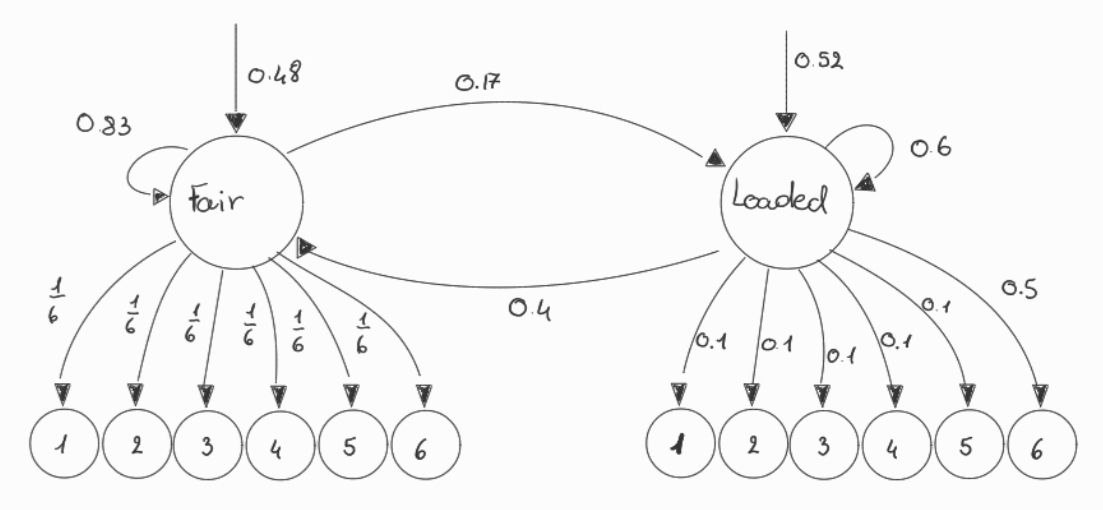
\includegraphics[width=.5\textwidth]{img/catene/dado.png}
                  \caption{Esempio di catena di Markov a stati nascosti}
                  \label{fig:dado}
              \end{figure}
              Supponiamo di voler calcolare la sequenza di stati più probabile
              data la sequenza di osservazioni $O = \{3, 1, 6, 6, 6, 4\}$. Possiamo
              utilizzare l'algoritmo di Viterbi per calcolare tale sequenza.
              Il funzionamento di tale algoritmo è riportato in figura \ref{fig:viterbi}.
              \begin{figure}[!ht]
                  \centering
                  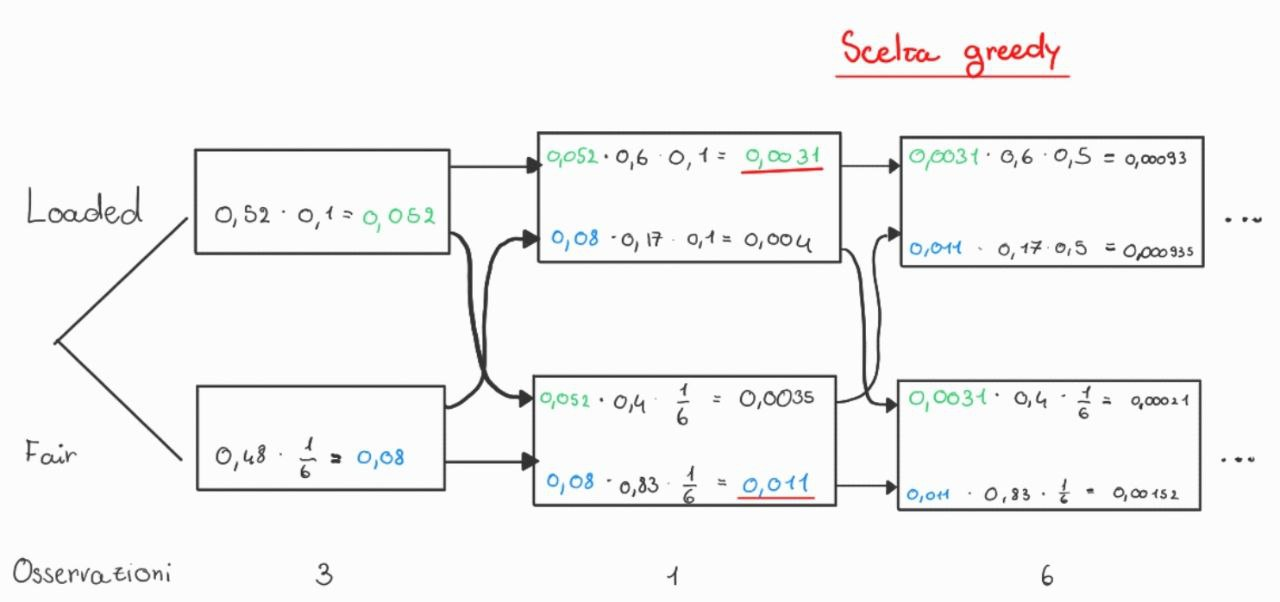
\includegraphics[width=.5\textwidth]{img/catene/viterbi.png}
                  \caption{Funzionamento dell'algoritmo di Viterbi}
                  \label{fig:viterbi}
              \end{figure}
              Infine, partendo dalla fine della sequenza, possiamo ricostruire la
              sequenza di stati più probabile seguendo le scelte greedy effettuate.
          \end{esempio}
\end{itemize}